\documentclass[11pt]{article}

\usepackage[a4paper,margin=1in]{geometry}
\usepackage{microtype}
\usepackage{amsmath,amssymb,amsfonts}
\usepackage{hyperref}
\usepackage{float}
\usepackage{placeins}
\usepackage{amsmath}
\usepackage{booktabs} 
\usepackage{array,booktabs,tabularx}
\usepackage{tikz}

% --- tables, floats, barriers ---
\usepackage{booktabs}     % for \toprule \midrule \bottomrule
\usepackage{array,tabularx}
\newcolumntype{L}{>{\raggedright\arraybackslash}X}
\usepackage{float}        % for [H]
\usepackage{placeins}     % for \FloatBarrier

% --- TikZ libraries used in figures ---
\usepackage{tikz}
\usetikzlibrary{calc,arrows.meta,positioning,decorations.pathreplacing}

% --- optional but useful cross-refs ---
\usepackage{hyperref}
\usepackage[nameinlink]{cleveref}

% --- notation helpers ---
\newcommand{\bell}{\boldsymbol\ell} % spatial projection vector
\newcommand{\clight}{c}             % speed of light macro

\usepackage{indentfirst}
\usetikzlibrary{arrows.meta,calc,angles,quotes}

\newcolumntype{L}{>{\raggedright\arraybackslash}X}
\newcommand{\sech}{\operatorname{sech}}


\numberwithin{equation}{section}

\title{Unimetry: A Phase-Space Reformulation of Special Relativity}
\author{Timur Abizgeldin\\ \small Independent researcher, Austria\\ \small \texttt{timurabizgeldin@gmail.com}}
\date{\today}


% --- Unimetry macros ---
\usepackage{tikz}
\usetikzlibrary{arrows.meta,positioning,calc}
\providecommand{\bi}{\mathbf{i}}
\providecommand{\bj}{\mathbf{j}}
\providecommand{\bk}{\mathbf{k}}
\providecommand{\uhat}{\hat{\mathbf u}}
\providecommand{\rotor}[2]{\cos\frac{#2}{2} + #1\,\sin\frac{#2}{2}}

\begin{document}
\maketitle
\begin{abstract}
We propose a compact reformulation of special relativity in which spacetime measures (time and length) are treated as phase velocities, defined as directional derivatives of a single underlying parameter, the flow $\boldsymbol{\chi}\in\mathbb{H}$. In this framework, the observable Minkowski interval emerges as a conserved quantity under a change of parameter from the phase coordinate $\chi$ to the observer’s proper time $\tau$. Familiar relativistic effects, such as time dilation, the Lorentz factor, the Doppler shift, and relativistic velocity composition, arise as elementary projections and rotations within a Euclidean phase plane. Hyperbolic features of Lorentz kinematics reappear after a reparametrization of time, yielding the classical relations without altering empirical content. We provide closed-form derivations for the longitudinal and transverse Doppler effects, prove a lemma equating the total flow speed to the conserved Minkowski norm, and outline connections to gauge phases, rapidity, and a cosmological time gauge. Composition of non-collinear boosts (quaternionic $d$-rotations in $\mathbb{H}$) yields a Wigner rotation; in the continuous limit, this gives Thomas precession. Both effects emerge as purely kinematical consequences of the quaternionic phase formalism. The approach is advantageous for applications – especially in modeling non-collinear acceleration of particle beams – where it replaces matrix diagonalizations with algebraic rotor compositions and improves numerical stability.
\end{abstract}

\paragraph{Keywords:} special relativity; phase; rapidity; Doppler shift; Lorentz factor; Wigner rotation; Thomas precession; phase parametrization.

\paragraph{MSC (2020):} 83A05; 70A05. % (Consider also PACS: 03.30.+p; 04.20.Cv.)

%1 ====================================================================

\section{Introduction}
In classical physics, space and time are taken as absolute and independent entities – a view deeply rooted in Newtonian tradition and characterizing most formulations prior to the early twentieth century. Special relativity revolutionized this perspective by demonstrating that both are intertwined and relative, depending on the observer’s state of motion. Yet most conventional treatments still regard spacetime coordinates as fundamental ingredients, with subsequent physical phenomena described in their terms.

This work adopts an alternative viewpoint: instead of starting from space and time as primitives, we treat observed spacetime quantities as derived projections of an underlying phenomenon – a continuous “flow” parameter $\boldsymbol{\chi}$ in quaternionic space $\mathbb{H}$. In this approach, the flow constitutes the primary structure, carrying both local geometric and dynamical information; observable temporal and spatial measures emerge from its decomposition relative to an observer’s frame.

This reformulation allows us to re-express relativistic effects – such as time dilation, Lorentz contraction, and the Doppler shift – as geometric consequences of rotations and projections in phase space, with quaternion algebra naturally unifying spatial rotations and boosts. The speed of light, in this setting, arises as the constant magnitude of the flow measured locally.

The proposal reorganizes familiar relations in a language aligned with quantum-rotor kinematics, demonstrating the physical equivalence between Lorentz transformations and Euclidean rotations under proper-time parametrization. We realize the phase kinematics with real quaternionic rotors.

Throughout, we use three angles – intrinsic ($\zeta$), gravitational ($\phi$), and kinematic ($\vartheta$) – and, when focusing on special relativity (SR), we state the corresponding simplification explicitly. We emphasize that no modification of Einstein’s dynamics is proposed; all results are kinematical identities obtained by a change of parameter.

\paragraph{Notation.} Tildes, dots, and primes denote derivatives with respect to the time-like parameter, proper time, and spatial arclength:
\[
\tilde{X}:=\frac{dX}{d\chi},\qquad \dot{X}:=\frac{dX}{d\tau},\qquad X':=\frac{dX}{dl}.
\]

\begin{table}[t]
\centering
\caption{Derivatives notation used in the paper.}
\label{tab:notation-phase}
\setlength{\tabcolsep}{6pt}\renewcommand{\arraystretch}{1.1}
\begin{tabularx}{\linewidth}{@{} l L @{}}
\toprule
\textbf{Symbol} & \textbf{Meaning} \\
\midrule
$\tilde{X}$ & $\chi$-parameter derivative with $\chi$ having time units; the (dimensionless) phase is $\Phi=\omega\,\chi$. \\
$\dot{X}$ & Proper-time derivative $dX/d\tau$ (lab-time derivatives are written $dX/dt$ explicitly). \\
$X'$ & Derivative with respect to spatial arclength $l$ or value in a primed inertial frame (as stated locally). \\
\bottomrule
\end{tabularx}
\end{table}

We use $\clight$ for the speed of light; $\beta:=v/\clight$, $\gamma:=1/\sqrt{1-\beta^2}$, and rapidity defined by $\tanh\eta=\beta$. The subscript $l$ in $dx_l$ denotes spatial components, with $l=1,2,3$ a Cartesian index.

%2 ====================================================================

\section{Flow concept}

% ================================Phase====================================

\subsection[Flow and phase 1-form]{Flow and phase 1-form}
Let $\Phi:\mathcal E\to\mathbb R$ be a scalar dimensionless phase potential on a Euclidean/Hilbert proto-space $(\mathcal E,\langle\cdot,\cdot\rangle)$, and the phase 1-form $\alpha:=d\Phi$. We use the normalized flow direction $\widehat{\boldsymbol\chi}:=\nabla\Phi/\|\nabla\Phi\|$ (when $\nabla\Phi\neq 0$), where the gradient is taken with respect to $\langle\cdot,\cdot\rangle$. The physical flow vector is fixed by the calibration in §\ref{sec:calibration-c} as $\boldsymbol\chi:=\clight \,\widehat{\boldsymbol\chi}$ (so $\|\boldsymbol\chi\|\equiv \clight$ thereafter).

Fix an observer’s orthonormal spatial triad $\{\mathbf e_1,\mathbf e_2,\mathbf e_3\}\subset\mathcal E$ and let $S=\mathrm{span}\{\mathbf e_1,\mathbf e_2,\mathbf e_3\}$ with orthogonal projectors $P_S$ and $P_{S^\perp}$. Decompose
\[
\boldsymbol\chi=\boldsymbol\chi_S+\boldsymbol\chi_\perp,\qquad
\boldsymbol\chi_S:=P_S\boldsymbol\chi,\quad 
\boldsymbol\chi_\perp:=P_{S^\perp}\boldsymbol\chi.
\]
Define observable spatial components and the orthogonal magnitude
\[
\ell_i:=\langle\boldsymbol\chi,\mathbf e_i\rangle,\qquad 
\mathbf l:=\sum_{i=1}^3 \ell_i\,\mathbf e_i,\qquad 
t_\perp:=\|\boldsymbol\chi_\perp\|=\sqrt{\|\boldsymbol\chi\|^2-\|\boldsymbol\chi_S\|^2},
\]
and, when $t_\perp>0$, the unit direction $\mathbf e_t:=\boldsymbol\chi_\perp/\|\boldsymbol\chi_\perp\|$.
Here $t_{\perp}$ always denotes the orthogonal flow magnitude $\|\boldsymbol\chi_\perp\|$, while $t$ denotes observer time throughout. 

Then the full phase angle $\Theta$ and the spatial direction $\mathbf u$ used throughout are
\[
\cos\Theta=\frac{t_\perp}{\|\boldsymbol\chi\|},\qquad 
\sin\Theta=\frac{\|\mathbf l\|}{\|\boldsymbol\chi\|},\qquad 
\mathbf u=\frac{\mathbf l}{\|\mathbf l\|}\quad(\|\mathbf l\|>0).
\]
Thus the observable space is a 3-manifold embedded in a (minimum) 4-dimensional flow manifold.

\begin{table}[!ht]
\centering
\caption{Notation for \S\;Flow and phase 1-form.}
\label{tab:flow-1form}
\setlength{\tabcolsep}{6pt}\renewcommand{\arraystretch}{1.1}
\begin{tabularx}{\linewidth}{@{} l L @{}}
\toprule
\textbf{Symbol} & \textbf{Meaning} \\
\midrule
$\mathcal E,\ \langle\cdot,\cdot\rangle,\ \|\cdot\|$ & Proto-space (Euclidean/Hilbert), its inner product, and the induced norm. \\
$\Phi:\mathcal E\to\mathbb R$ & Scalar \emph{phase potential}. \\
$\alpha:=d\Phi$ & Phase 1-form (exact differential of $\Phi$). \\
$\widehat{\boldsymbol\chi}:=\nabla\Phi/\|\nabla\Phi\|$  &  Normalized flow direction (when $\nabla\Phi\neq0$). Physical flow: $\boldsymbol\chi:=\clight \,\widehat{\boldsymbol\chi}$. \\
$\{\mathbf e_1,\mathbf e_2,\mathbf e_3\}$ & Observer’s orthonormal spatial triad. \\
$S=\mathrm{span}\{\mathbf e_1,\mathbf e_2,\mathbf e_3\}$ & Observable 3-space; $S^\perp$ is its orthogonal complement. \\
$P_S,\ P_{S^\perp}$ & Orthogonal projectors onto $S$ and $S^\perp$. \\
$\boldsymbol\chi_S:=P_S\boldsymbol\chi,\ \ \boldsymbol\chi_\perp:=P_{S^\perp}\boldsymbol\chi$ & Decomposition of the flow into spatial and orthogonal parts ($\boldsymbol\chi=\boldsymbol\chi_S+\boldsymbol\chi_\perp$). \\
$\ell_i:=\langle\boldsymbol\chi,\mathbf e_i\rangle$ & Scalar components of the flow along the triad. \\
$\mathbf l:=\sum_{i=1}^3 \ell_i\,\mathbf e_i$ & Observable spatial projection of the flow ($\mathbf l\equiv\boldsymbol\chi_S$). \\
$t_\perp:=\|\boldsymbol\chi_\perp\|=\sqrt{\|\boldsymbol\chi\|^2-\|\boldsymbol\chi_S\|^2}$ & Orthogonal (“temporal-fiber”) magnitude. \\
$\mathbf e_t:=\boldsymbol\chi_\perp/\|\boldsymbol\chi_\perp\|$ & Unit direction along $S^\perp$ (defined when $t_\perp>0$). \\
$\Theta$ & Full phase angle defined by $\cos\Theta=\dfrac{t_\perp}{\|\boldsymbol\chi\|}$ and $\sin\Theta=\dfrac{\|\mathbf l\|}{\|\boldsymbol\chi\|}$. \\
$\mathbf u:=\mathbf l/\|\mathbf l\|$ & Unit spatial direction of the flow (defined when $\|\mathbf l\|>0$). \\
\midrule
— & With these definitions, the observable space $S$ is a 3-manifold embedded in a (minimum) 4-dimensional flow manifold $S\oplus\mathrm{span}\{\mathbf e_t\}$. \\
\bottomrule
\end{tabularx}
\end{table}

% ============================Flow========================================

\subsection{Flow description}\label{sec:flow}

In the flow-based description an object is a collection of elementary “streamlets” (fragments of total object phase flow). Each streamlet admits a co-moving frame in which its spatial projection vanishes and its budget angle equals zero in that frame (``self time'' direction).

Larger stable streamlets combinations are Newtonian bodies, which are formed by multiple “self time” flows equally spreaded over the body's 3-surface. Therefore, unlike streamlets bodies have generalized time axis - their time flow isn't already geometric phenomenon.

\emph{Postulate}. From the ability of bodies to preserve a place within the observable space, we conclude the cyclical nature of streamlets' flows in $\mathcal E$:

\begin{equation}
\oint{\alpha} = 2\pi.
\label{eq:alpha-cycle}
\end{equation}

% ============================Body========================================

\subsection{Flow of a complex body}\label{sec:body}

Let a (Newtonian) body $B$ be a finite–energy ensemble of streamlets $\mathcal A=\{a\}$ with flows $\boldsymbol\chi_a$, phase angles $\Theta_a$, and (when defined) unit spatial directions $\mathbf u_a\in S$. Assign non-negative weights $w_a$ (fraction of the body's rest energy carried by $a$) with $\sum_a w_a=1$, and impose the rest–balance condition
\begin{equation}
\sum_{a\in\mathcal A} w_a\,\boldsymbol\chi_{S,a}=0,
\qquad \oint \alpha_a = 2\pi \quad \text{(cycle postulate).}
\label{eq:body-balance}
\end{equation}

Because a body does not possess a single geometric time axis (its streamlets’ self–time directions $\mathbf e_{t,a}$ are distributed), the effective temporal and spatial responses must be understood statistically. We therefore introduce the scalar temporal coefficient and the spatial shape tensor (second moment) as
\begin{equation}
T_B:=\sum_a w_a \cos^2\Theta_a,
\qquad
\mathbf C_B:=\sum_a w_a\,\sin^2\Theta_a\; \mathbf u_a\!\otimes\!\mathbf u_a,
\label{eq:TB-CB}
\end{equation}
where $0<T_B\le 1$ and $\mathbf C_B$ is a symmetric positive semidefinite
tensor on $S$ with $\mathrm{tr}\,\mathbf C_B=\sum_a w_a \sin^2\Theta_a$.
Operationally, $T_B$ captures the aggregate fraction of flow carried in the
orthogonal (self–time) fiber, while $\mathbf C_B$ encodes the anisotropic
distribution of spatial projections across the body's 3-surface.

With these ensemble quantities we define the body's \emph{proper time
increment} by
\begin{equation}
d\tau_B:=\sqrt{T_B}\, d\chi,
\label{eq:body-proper-time}
\end{equation}
and the body's \emph{self spatial quadratic form} on $S$ by
\begin{equation}
q_B(d\mathbf \ell):= d\mathbf \ell^{\!\top}\mathbf C_B\,d\mathbf \ell .
\label{eq:body-spatial-form}
\end{equation}

This yields a natural candidate for the body's \emph{self metric} as a
quadratic form on $(d\chi,d\mathbf \ell)$:
\begin{equation}
ds_B^2 \;:=\; \clight^2\, d\tau_B^2 \;-\; q_B(d\mathbf \ell)
\;=\; \clight^2 T_B\, d\chi^2 \;-\; d\mathbf \ell^{\!\top}\mathbf C_B\,d\mathbf \ell .
\label{eq:body-self-metric}
\end{equation}

In the isotropic rest configuration (identical $\Theta_a$ and uniform
$\mathbf u_a$ on $S^2$) one has $\mathbf C_B=\tfrac{\sin^2\Theta}{3}\,\mathbf
I_S$, so \eqref{eq:body-self-metric} reduces to the standard Minkowski form
up to the overall phase gauge $d\chi$; fixing the gauge by $T_B\equiv 1$ at
rest makes $d\tau_B=d\chi$ and restores $q_B(d\mathbf \ell)=\|d\mathbf
\ell\|^2$. Away from isotropy, $\mathbf C_B$ becomes ellipsoidal, and the
body’s proper metric records the internal orientation texture of its
streamlets.

The next section formalizes \eqref{eq:body-self-metric}, shows how external
kinematics (the angle $\vartheta$) and additional phase tilts (intrinsic
$\zeta$, gravitational $\phi$) renormalize $(T_B,\mathbf C_B)$, and derives
the usual relativistic effects as deformations of the ensemble moments
\eqref{eq:TB-CB}.

% ============================Calibration========================================
\subsection{Local calibration by the invariant signal speed}\label{sec:calibration-c}

The cycle postulate \eqref{eq:alpha-cycle} fixes the phase scale of each streamlet, but leaves an overall unit choice for the flow magnitude $\|\boldsymbol\chi\|$. We now calibrate this scale operationally by the invariant signal speed $\clight$.

\emph{Calibration postulate (vacuum, isotropic texture).}
There exist null excitations (``lightlike'' streamlets) for which the body-level proper increment vanishes, $d\tau_B=0$ (equivalently $T_B=0$), and whose spatial advance per phase increment is direction–independent in vacuum. We define the numerical value of $\clight$ by the rule
\begin{equation}
\frac{\|d\boldsymbol\ell\|}{d\chi}=\clight
\qquad\text{along null flow lines in vacuum.}
\label{eq:calib-null}
\end{equation}

\paragraph{Flow-norm gauge.}
For any elementary flow, the Euclidean split gives $\|\boldsymbol\chi\|^2=\|\boldsymbol\chi_S\|^2
+\|\boldsymbol\chi_\perp\|^2$. Along a null flow (orthogonal share vanishes) we have
$\|\boldsymbol\chi\|=\|\boldsymbol\chi_S\|=\|d\boldsymbol\ell\|/d\chi$; combining with
\eqref{eq:calib-null} fixes the flow-norm gauge
\begin{equation}
\boxed{\ \|\boldsymbol\chi\|\equiv \mathtt c\ }.
\label{eq:flow-norm-c}
\end{equation}
Consequently, for any decomposition angle $\Theta$ introduced in \S\;Flow and phase 1-form,
\begin{equation}
\|\boldsymbol\chi_S\|=\clight\,\sin\Theta,\qquad
\|\boldsymbol\chi_\perp\|=\clight\,\cos\Theta.
\label{eq:proj-calibrated}
\end{equation}

\paragraph{Ensemble consequences.}
For a body $B$ the second moments \eqref{eq:TB-CB} read, after the gauge
\eqref{eq:flow-norm-c},
\begin{equation}
T_B=\sum_a w_a\cos^2\Theta_a,\qquad
\mathrm{tr}\,\mathbf C_B=\sum_a w_a\sin^2\Theta_a=1-T_B,
\end{equation}
and the intrinsic metric \eqref{eq:body-self-metric} becomes
\begin{equation}
\boxed{\ ds_B^2=\clight^2 T_B\,d\chi^2 - d\bell^{\!\top}\mathbf C_B\,d\bell\ }.
\end{equation}
Thus $\clight$ is not introduced dynamically but arises as the \emph{fixed magnitude of the
flow} under the calibration \eqref{eq:calib-null}; tilts rotate the budget between the two
projections without changing $\|\boldsymbol\chi\|$.

\paragraph{Units and phase (resolution of dimensions).}
We adopt $\chi$ as a time-like parameter and define the (dimensionless) phase by $\Phi=\omega\,\chi$,
so that $\alpha=d\Phi=\omega\,d\chi$. The cycle postulate $\oint\alpha=2\pi$ then implies
$\oint d\chi=2\pi/\omega$ along a closed loop. In particular, for null flows in vacuum our
calibration $\|d\bell\|/d\chi=\clight$ fixes the affine advance of $\chi$ per emitted cycle via the
emission frequency~$\omega$.

\paragraph{Invariance under uniform tilts.}
A uniform phase tilt acts as $\Theta_a\mapsto\Theta_a+\delta$ (see \S\ref{sec:intrinsic-angle}
below). It preserves the norm \eqref{eq:flow-norm-c} and merely redistributes the
projections as in \eqref{eq:proj-calibrated}. Hence $\clight$ is invariant, while $T_B$ and
$\mathbf C_B$ renormalize.

% ============================Intrinsic angle========================================
\subsection{Intrinsic angle}\label{sec:intrinsic-angle}

Using the ensemble second moments \eqref{eq:TB-CB}, define
\[
C:=\sum_a w_a\cos 2\Theta_a,\qquad S:=\sum_a w_a\sin 2\Theta_a .
\]
There exists a unique $\zeta\in[0,\tfrac{\pi}{2}]$ such that
\begin{equation}
(\cos 2\zeta,\ \sin 2\zeta)=(C,S)
\quad\Longleftrightarrow\quad
T_B=\tfrac12(1+C)=\cos^2\!\zeta,\qquad
\operatorname{tr}\mathbf C_B=\tfrac12(1-C)=\sin^2\!\zeta .
\label{eq:zeta-def}
\end{equation}
We call $\zeta$ the \emph{effective (intrinsic) angle}: it aggregates the temporal/spatial budget at the level relevant for the intrinsic metric \eqref{eq:body-self-metric}. In particular,
\[
d\tau_B=\cos\zeta\,d\chi,\qquad
ds_B^2=\clight^2\cos^2\!\zeta\,d\chi^2-d\boldsymbol\ell^{\!\top}\mathbf C_B\,d\boldsymbol\ell,
\]
and for an isotropic texture $\mathbf C_B=\tfrac{\sin^2\!\zeta}{3}\,\mathbf I_S$.

\paragraph{Why the double angle.}
Since $ds_B^2$ depends only on $\cos^2\Theta_a$ and $\sin^2\Theta_a$, we linearize the ensemble average via
$\cos^2\Theta=\frac12(1+\cos2\Theta)$ and $\sin^2\Theta=\frac12(1-\cos2\Theta)$, and collect
$(C,S)=\sum_a w_a(\cos2\Theta_a,\sin2\Theta_a)$. Then $\zeta=\tfrac12\mathrm{atan2}(S,C)$ ensures $T_B=\cos^2\zeta$ and makes a uniform tilt $\Theta_a\mapsto\Theta_a+\delta$ act additively: $\zeta\mapsto\zeta+\delta$.

\paragraph{Uniform tilt mechanism.}
A uniform phase tilt by $\delta$ transforms
\[
C(\delta)=C\cos2\delta - S\sin2\delta,\qquad
S(\delta)=C\sin2\delta + S\cos2\delta,
\]
hence
\begin{equation}
\zeta\ \longmapsto\ \zeta'=\zeta+\delta,\qquad
T_B(\delta)=\cos^2(\zeta+\delta),\qquad
\operatorname{tr}\mathbf C_B(\delta)=\sin^2(\zeta+\delta),
\label{eq:zeta-tilt}
\end{equation}
while the full spatial texture remains $\mathbf C_B(\delta)=\sum_a w_a\sin^2(\Theta_a+\delta)\,\mathbf u_a\otimes\mathbf u_a$ (isotropy is preserved by a uniform tilt).

\medskip
Equations \eqref{eq:body-self-metric}–\eqref{eq:zeta-tilt} complete the object-level construction:
the body observes the quadratic geometry $ds_B^2$, fully controlled by $(\zeta,\mathbf C_B)$.
Relative measurements between two bodies will be introduced later via their shadows in $S$.

% --- PATCH A: insert at the end of § Intrinsic angle, after eq. \eqref{eq:zeta-tilt} ---

\paragraph{Remark (symmetric phase pair and nonvanishing spatial share).}
A frequently used mnemonic for a nonvanishing spatial projection is to pair opposite tilts
\[
\boldsymbol{\chi}^{\pm}=R\,e^{\pm\zeta\,\mathbf{l}},\qquad
\boldsymbol{\chi}_l:=\frac{\boldsymbol{\chi}^+-\boldsymbol{\chi}^-}{2}
=R\,\mathbf{l}\,\sin\zeta ,
\]
which matches the decomposition
$\boldsymbol{\chi}_0=\boldsymbol{\chi}_\tau+\boldsymbol{\chi}_l
=R\cos\zeta+R\,\mathbf{l}\sin\zeta$.
In the ensemble language of \eqref{eq:TB-CB}, this construction is not a new
dynamics but merely a parametrization of the \emph{second moments}:
the spatial budget enters through $\sin^2\Theta_a$ and is fully captured by
$\operatorname{tr}\mathbf C_B=\sin^2\zeta$ in \eqref{eq:zeta-def}.
Uniform tilts act additively on the effective angle $\zeta$ as in \eqref{eq:zeta-tilt}.


% ==================================Angles==================================
\subsection[Three angles]{Three angles}
\label{subsec:three-angles}

We will use three angles with distinct roles:

\begin{itemize}
  \item \textbf{Intrinsic angle} $\boldsymbol{\zeta}\in[0,\tfrac{\pi}{2}]$:
  a second-moment budget angle of the body (no geometric time axis).
  It is defined by $T_B=\cos^2\zeta$ from \eqref{eq:zeta-def} and governs the intrinsic rate
  via $d\tau_B=\cos\zeta\,d\chi$. When the same flow characterizes a background medium
  (not the photon itself), its optical response can be encoded by
  \[
    v_{\mathrm{ph}}(\text{medium})=\clight\,\cos\zeta,\qquad
    n(\zeta)=\frac{\clight}{v_{\mathrm{ph}}}=\sec\zeta,
  \]
  while in the local phase chart ($dt:=d\chi$) one has $d\tau_B/dt=\cos\zeta$.
  \emph{Note:} $\zeta$ is a scalar second-moment parameter, not linked to a direction.

  \item \textbf{Gravitational angle} $\boldsymbol{\phi}$:
  an external tilt field that uniformly rotates streamlet budgets
  (cf.\ \eqref{eq:zeta-tilt}). In the weak, stationary regime it reproduces
  clock slowing and light delay through an effective index
  $n_g=\sec\phi$ and $d\tau/dt=\cos\phi$ (no field equations assumed here).
  Uniform tilts add on second moments, so $\zeta$ and $\phi$ combine as $\zeta\mapsto\zeta+\phi$.

  \item \textbf{Kinematic angle} $\boldsymbol{\vartheta}$:
  an \emph{observer–relative} directional tilt (introduced in §\ref{sec:minkowski-derivation})
  built from an observer’s split and the unit flow direction. It parameterizes
  relative motion between bodies; in the SR simplification (below) it becomes the
  sole angle.
\end{itemize}

% ==================================Simplification==================================
\subsection[SR simplification]{SR simplification}
\label{subsec-1-5-sr-simplification}

Whenever along a worldline segment two bodies share the same intrinsic and gravitational
tilts (i.e.\ $\zeta_A=\zeta_B$ and $\phi_A=\phi_B$), one can choose a local comoving chart
in which only the directional (kinematic) tilt matters. In SR–focused passages we
\emph{set} $\zeta=\phi=0$ and use $dt:=d\chi$; then the kinematic angle $\vartheta$ is the
only parameter. The standard relations (e.g.\ the Minkowski interval and the familiar
speed/rate identities) will be derived in the next subsection from this setting.


% ============================Minkowski metric derivation========================================
\subsection[Minkowski metric derivation]{Minkowski metric derivation}\label{sec:minkowski-derivation}

Let $A$ be an observer with orthonormal spatial triad $\{\mathbf e_1^A,\mathbf e_2^A,\mathbf e_3^A\}$,
$S^A=\mathrm{span}\{\mathbf e_i^A\}$, and time direction $\mathbf e_t^A\parallel (S^A)^\perp$.
For an object with unit flow direction $\widehat{\mathbf F}:=\boldsymbol\chi/\|\boldsymbol\chi\|$,
define the \emph{observer–object} angle by
\[
\widehat{\mathbf F}
= \cos\vartheta_{\,\!|\!A}\,\mathbf e_t^A
+ \sin\vartheta_{\,\!|\!A}\,\mathbf u_{\,\!|\!A},\qquad
\mathbf u_{\,\!|\!A}:=\frac{P_{S^A}\widehat{\mathbf F}}{\|P_{S^A}\widehat{\mathbf F}\|}\in S^A .
\]
\paragraph{Angle roles (no self time-axis for a composite).}
For a composite body the intrinsic angle $\zeta$ is a second-moment scalar (budget of temporal vs.\ spatial shares) entering $ds_B^2$, not a direction. Hence the body has no geometric self time-axis, and there is no notion of “being collinear” with $\mathbf e_t^A$. The observer–object angle $\vartheta_{|\!A}$ is purely directional (built from $A$’s split and $\widehat{\mathbf F}$), while $\zeta$ controls the intrinsic rate via $T_B=\cos^2\zeta$; they are conceptually independent.


\paragraph{Calibration for the SR sector.}
To compare with the laboratory rulers in $A$’s frame without invoking any dynamics, we fix a purely
kinematic \emph{SR sector}:
\begin{enumerate}\itemsep4pt
\item intrinsic and gravitational tilts are switched off: $\zeta=\phi=0$ (so $T_B=1$ in the rest state);
\item the body’s spatial texture is isotropic in its rest configuration: $\mathbf C_B\propto\mathbf I_S$;
\item we take $A$’s lab chart as the phase chart: $dt_A:=d\chi$.
\end{enumerate}
With these conventions, the spatial increment seen by $A$ is
\[
d\mathbf x_{\,|\!A}=\clight\,\sin\vartheta_{\,\!|\!A}\,dt_A\,\mathbf u_{\,\!|\!A},
\]
and the object’s proper time equals the phase chart in this sector: $d\tau_B=d\chi=dt_A$.
By $\cos^2+\sin^2=1$ we obtain the Minkowski interval in $A$’s rulers:
\begin{equation}
\boxed{\ \clight^2\,d\tau_B^2 \;=\; \clight^2\,dt_A^2 \;-\; \|d\mathbf x_{\,|\!A}\|^2\ }\quad
\text{(SR sector: $\zeta=\phi=0$, isotropic rest, $dt_A=d\chi$).}
\end{equation}

\paragraph{Remark (outside the SR sector).}
For general $(\zeta,\mathbf C_B)$ the intrinsic interval is always
$ds_B^2=\clight^2 T_B\,d\chi^2-d\boldsymbol\ell^{\!\top}\mathbf C_B\,d\boldsymbol\ell$.
Expressing this in $A$’s lab chart ($dt_A=d\chi$) yields direction-dependent pullbacks via
$\mathbf C_B$; the standard Minkowski form is recovered precisely when the SR-sector
assumptions above hold. The relative (“two-body”) kinematics and the emergence of familiar
SR effects will be introduced later by comparing the shadows of two objects.


% ============================Symmetry========================================
\subsection[Symmetry]{Symmetry}

\paragraph{Two bodies ($A$ and $B$).}
Repeating the calibrated SR-sector construction in $B$’s frame gives the same interval form in $B$’s
rulers. Swapping “who projects whom” exchanges the splits $(\mathbf e_t^A,S^A)\leftrightarrow(\mathbf e_t^B,S^B)$ but leaves the Minkowski form invariant.

%3 ====================================================================

\section[Operations]{Operations}

% ================================Quaternions====================================

\subsection[Why quaternion algebra]{Why quaternion algebra}
\label{subsec-1-2-why-quaternion-algebra}
Quaternions form the minimal non-commutative algebra that (i) double-covers $SO(3)$ for rigid 3D rotations; (ii) carries the Hopf fibration $S^3\to S^2$, separating an internal $S^{1}$ time fiber from spatial orientations; and (iii) encodes the non-commutativity responsible for Wigner–Thomas rotations (residual spatial rotations from composing non-collinear boosts) \cite{Hopf1931,Wigner1939,Thomas1926}.

Simply put one standard sandwich operation in $\mathbb{H}$ of the kind: $\hat{q} \rightarrow \hat{r}_1\hat{q}\hat{r}_2$; is sufficient to perform any possible rotation on $S^3$; the quaternion algebra then simplifies operations on flows relative to the lab triad.

\paragraph{Why a complex slice of a quaternion?}
For local kinematics any unit direction $\hat{\mathbf u}$ singles out the two-dimensional subalgebra $\mathrm{Span}\{1,\hat{\mathbf u}\}\cong\mathbb{C}\subset\mathbb{H}$. Working in this complex slice preserves the boost/rotation algebra along $\hat{\mathbf u}$ while keeping formulas elementary. When the direction changes, the slice is updated; the full quaternionic structure is retained.

% ================================The spatially linked quaternion====================================

\subsection[The spatially linked quaternion]{The spatially linked quaternion}
\label{subsec:spatialq}
At a point $P\in S$, define
\[
q:=t_\perp+\mathbf l \;=\; t_\perp+l_1\,\mathbf i+l_2\,\mathbf j+l_3\,\mathbf k,
\qquad
\|q\|^2=t_\perp^2+\|\mathbf l\|^2=\|\boldsymbol\chi\|^2,
\qquad
\widehat q := \frac{q}{\|q\|}.
\]

Hence $\widehat q\in S^3\simeq SU(2)$ encodes the lab-linked state, and a convenient calibration is $\|\boldsymbol\chi\|=\clight$, so that $\|q\|=\clight$.

Let the observed object internal imaginary basis be $\{I,J,K\}\subset\Im\mathbb H$. The observed (lab) orthonormal triad is the conjugated image
\[
\mathbf e_{\mathbf i}(\widehat q)=\widehat q\, I \,\widehat q^{-1},\qquad 
\mathbf e_{\mathbf j}(\widehat q)=\widehat q\, J \,\widehat q^{-1},\qquad 
\mathbf e_{\mathbf k}(\widehat q)=\widehat q\, K \,\widehat q^{-1}.
\]

Therefore, it's claimed that the quaternion field over the observable 3D-space manifold defines the direction of the object flow relatively to the lab frame. Considering the time cyclical we introduce the \emph{time fiber} generated by right multiplication with $e^{\frac{\sigma}{2}K}$; its spatial director (shadow) is $\mathbf n(\widehat q)=\widehat q K \widehat q^{-1}\in S^2$. This gives a potential link to quantum mechanics spheres.


\subsection{Velocity addition} \label{sec:vel-addition}
\paragraph{Notation.} In unimetry, an inertial boost is a \emph{D-rotation}
\begin{equation} \label{eq:auto:32}
\mathcal{B}(\uhat,\psi):\quad \mathbf q \mapsto d\,\mathbf q\,d, \qquad d=\cos\frac{\psi}{2}+\uhat\,\sin\frac{\psi}{2},
\end{equation}
and a spatial rotation is an \emph{R-rotation}
\begin{equation} \label{eq:auto:33}
\mathcal{R}(\hat{\mathbf n},\varphi):\quad \mathbf q \mapsto r\,\mathbf q\,r^{-1}, \qquad r=\cos\frac{\varphi}{2}+\hat{\mathbf n}\,\sin\frac{\varphi}{2}.
\end{equation}
Kinematic mapping: $\beta\equiv \mathbf v/ \clight=\sin\psi$, $\gamma=1/\cos\psi$, $\displaystyle \tan\frac{\psi}{2}=\frac{\gamma\beta}{\gamma+1}$. For quaternionic/GA accounts of rotors and Lorentz boosts see \cite{Hamilton1844,HestenesSobczyk1984,DoranLasenby2003}.

\subsubsection{Wigner rotation} \label{subsec:wigner}
Let $d_1,d_2$ be D-rotors of two successive boosts. The raw action on any unimetry 4-object is
\begin{equation} \label{eq:auto:34} \mathbf q' = d_2 d_1\, \mathbf q\, d_1 d_2 \equiv L_{12}\,\mathbf q\,L_{21},\qquad L_{12}=d_2 d_1,\ \ L_{21}=d_1 d_2.
\end{equation}
Define $d_{12}$ to be the unique D-rotor reproducing the combined spatio--temporal tilt of $L_{12}$:
\begin{equation} \boxed{\, d_{12}\,\mathbf e_t\, d_{12} \;=\; L_{12}\,\mathbf e_t\, L_{21},\qquad \Re(d_{12})\ge0 \,} \label{eq:d12-uniqueness}
\end{equation}
(the sign choice removes the trivial two-fold ambiguity). Then the Wigner rotor is the residual R-rotation in the symmetric D--R factorization:
\begin{equation}
\boxed{\, L_{12}=d_{12}\,r_W,\qquad L_{21}=r_W^{-1}\,d_{12} \,} \label{eq:DR-polar}
\end{equation}
equivalently,
\begin{equation} \boxed{\, r_W=\bar d_{12}\,L_{12}=L_{21}\,\bar d_{12} \,}. \label{eq:wigner-rotor-def}
\end{equation}
Hence the observed map after compensating the tilt is $\,\bar d_{12}\,\mathbf q'\,\bar d_{12}=r_W\,\mathbf q\,r_W^{-1}$.
\begin{figure}[!ht] \centering
\begin{tikzpicture}[>=Latex, node distance=32mm] \node (q) {$\mathbf q$}; \node (d1) [right=of q] {$d_1\,\mathbf q\,d_1$}; \node (d2) [right=of d1] {$d_2 d_1\,\mathbf q\,d_1 d_2$}; \node (rw) [below=20mm of d2] {$r_W\,\mathbf q\,r_W^{-1}$}; \draw[->] (q) -- node[above] {$d_1$} (d1); \draw[->] (d1) -- node[above] {$d_2$} (d2); \draw[->] (d2) -- node[right] {$\bar d_{12}$ on both sides} (rw); \draw[->, dashed, bend left=12] (q) to node[above] {$d_{12}$} (d2); \end{tikzpicture} \caption{Two successive D-rotations (boosts) and compensation of the net spatio--temporal angle by the conjugate of $d_{12}$, leaving a pure R-rotation $r_W$.} \label{fig:tikz-wigner-pullback} \end{figure} \subsubsection{Thomas precession} \label{subsec:thomas} The continuous limit of Wigner rotation for a time-dependent velocity direction $\uhat(t)$ yields \begin{equation} \label{eq:auto:38} \boldsymbol{\omega}_T=(\gamma-1)\,\bigl(\uhat\times \dot{\uhat}\bigr) =\frac{\gamma^2}{\gamma+1}\,\frac{\mathbf a\times \mathbf v}{c^2},\qquad \gamma=\frac{1}{\cos\psi}. \end{equation} For uniform circular motion ($|\mathbf v|=\mathrm{const}$) with $\dot{\uhat}=\boldsymbol{\Omega}\times\uhat$ one has $\lvert\boldsymbol{\omega}_T\rvert=(\gamma-1)\,\Omega$.


\subsection{Time fiber, Hopf fibration, and the Bloch/Poincaré spheres.}
Consider the map $\pi:S^3\simeq SU(2)\to S^2$ given by
\[
\pi(q)\;=\;\mathbf n(q)\;:=\;q\,K\,q^{-1},
\]
where $K\in\Im\mathbb H$ is a fixed internal unit (the reference “time-axis” in the internal frame). Then:

\emph{(i) $U(1)$ fiber by right action.}
For any $\sigma\in\mathbb R$,
\[
\mathbf n\!\big(q\,e^{\frac{\sigma}{2}K}\big)
= q\,e^{\frac{\sigma}{2}K}\,K\,e^{-\frac{\sigma}{2}K}\,q^{-1}
= q\,K\,q^{-1}
= \mathbf n(q),
\]
since $K$ commutes with $e^{\frac{\sigma}{2}K}$. Thus the set
\[
\mathcal F_{\,\mathbf n}\;=\;\big\{\,q\,e^{\frac{\sigma}{2}K}\;:\;\sigma\in[0,2\pi)\big\}
\]
is the $U(1)$ fiber over the base point $\mathbf n\in S^2$. In our kinematics, this right $U(1)$ action is the \emph{time fiber}: internal evolution that preserves the observed spatial director.

\emph{(ii) Surjectivity and $S^2$ base.}
For any unit $\mathbf n\in\Im\mathbb H$ there exists $q\in SU(2)$ with $q\,K\,q^{-1}=\mathbf n$ (double cover $SU(2)\to SO(3)$). Hence the base of the fibration is the 2-sphere $S^2$ of spatial directions.

\emph{(iii) Link to quantum spheres.}
Identifying $\Im\mathbb H\simeq\mathfrak{su}(2)$ (and, via Pauli matrices, with $\mathbb R^3$), the map 
\[
\mathbf n(q)=q\,K\,q^{-1}
\]
is the quaternionic form of the Bloch vector for a qubit, or the Stokes vector on the Poincaré sphere for polarization: normalized state rays $(\psi\in\mathbb C^2,\ \|\psi\|=1)$ modulo global phase $U(1)$ correspond to points on $S^2$. Thus $S^3/U(1)\cong S^2$ is the familiar “state-ray” geometry; our time fiber is the same $U(1)$ that is unobservable as a global phase in standard QM, but becomes a \emph{kinematic} degree of freedom here.

\emph{(iv) Geometric phase.}
If $q(\tau)$ traces a loop whose shadow $\mathbf n(\tau)$ makes a closed path on $S^2$, parallel transport in the $U(1)$ fiber accumulates a Berry‐type phase $\gamma=\tfrac{1}{2}\Omega[\mathbf n]$, half the solid angle enclosed by the loop on the sphere. In our setting this is an \emph{internal time} holonomy: purely kinematic and arising from the bundle connection induced by the Hopf fibration.

\paragraph{Remark.}
Left–conjugation $v\mapsto q\,v\,q^{-1}$ rotates lab vectors (changes the \emph{base} point on $S^2$), whereas right multiplication by $e^{\frac{\sigma}{2}K}$ moves along the \emph{fiber} at fixed $\mathbf n$. This cleanly separates spatial reorientation from internal (time/phase) evolution.



%3 ===================================================================

\section{\texorpdfstring{Phase: operational definition and physical meaning}{Phase: operational definition and physical meaning}}\label{sec:operational-phase}
% --- patch: angle motivation ---
We will systematically replace hyperbolic functions and nested square roots by the circular trigonometry of a single \emph{phase angle} $\vartheta$, interpreting $\cos\vartheta$ as the temporal projection and $\sin\vartheta$ as the spatial one. This keeps all kinematic identities while avoiding hyperbolic parametrization.  

\emph{Convention.} In this section we track a single body, so $\tau\equiv\tau_B$.

We define the \emph{kinematic angle} $\vartheta\in[0,\tfrac{\pi}{2})$ of a system with respect to a fixed observer as an \textbf{operationally measurable split} of a constant ``flow budget'' $\clight$ between temporal and spatial projections:
\begin{equation}
\boxed{\quad \cos\vartheta \equiv \frac{d\tau}{dt}, \qquad \sin\vartheta \equiv \frac{\|\mathbf v\|}{\clight}=\beta, \quad \mathbf{u}=\frac{\mathbf v}{\|\mathbf v\|}\quad}
\label{eq:operational-phase}
\end{equation}
where $t$ is the observer's time, $\tau$ is the proper time, and $\mathbf v$ is the 3-velocity. The identity $\cos^2\vartheta+\sin^2\vartheta=1$ then restates the empirical invariance of the Minkowski interval.

\paragraph{Phase state and quaternionic slice.}
An (inertial) phase state is the pair $(\vartheta,\mathbf u)$, with $\mathbf u\in S^2$. We associate to it the unit quaternion
\begin{equation}
q(\vartheta,\mathbf u)=\cos\vartheta + \mathbf u\,\sin\vartheta, \qquad 
\mathbf u:=u_x\,\mathbf i+u_y\,\mathbf j+u_z\,\mathbf k, \ \ \|\mathbf u\|=1,
\end{equation}
that is, a complex slice $\mathbb C_{\mathbf u}:=\mathrm{Span}\{1,\mathbf u\}\subset\mathbb H$ aligned with $\mathbf u$. This is the minimal structure that linearly encodes collinear compositions and naturally induces the Wigner--Thomas rotation for non-collinear boosts via quaternion multiplication.

%3 ===================================================================

\section{\texorpdfstring{Mapping to standard SR variables}{Mapping to SR}}
The phase angle $\vartheta$ is \emph{not} the rapidity $\eta$; they are related by a Gudermann-type~\cite{Gudermann1830} bridge
\begin{equation}
\boxed{\ \ \beta=\tanh\eta=\sin\vartheta,\qquad \gamma=\cosh\eta=\sec\vartheta,\qquad 
\tan\frac{\vartheta}{2}=\tanh\frac{\eta}{2}\ \ }.
\label{eq:gudermann}
\end{equation}

Consequently, all standard kinematic relations follow from circular trigonometry in $\vartheta$:
\begin{equation}
\gamma=\frac{1}{\sqrt{1-\beta^2}}=\sec\vartheta,\qquad 
k_{\parallel}=e^{\pm\eta}=\frac{1+\tan(\vartheta/2)}{1-\tan(\vartheta/2)}.
\end{equation}

All collinear compositions reduce to angle addition inside the slice $\mathbb{C}_{\mathbf u}$.

\paragraph{Collinear composition.}
For $\mathbf u$ fixed,
\begin{equation}
q(\vartheta_2,\mathbf u)\,q(\vartheta_1,\mathbf u)=q(\vartheta_1\oplus\vartheta_2,\mathbf u),\qquad 
\cos(\vartheta_1\oplus\vartheta_2)=\cos\vartheta_1\cos\vartheta_2-\sin\vartheta_1\sin\vartheta_2,
\end{equation}
which implies Einstein's velocity addition
\begin{equation}
\beta_{12}=\sin(\vartheta_1\oplus\vartheta_2)=\frac{\beta_1+\beta_2}{1+\beta_1\beta_2}.
\end{equation}

\paragraph{Non-collinear composition and Wigner--Thomas rotation.}
For $\mathbf u_1\neq\mathbf u_2$ one has the factorization
\begin{equation}
q(\vartheta_2,\mathbf u_2)\,q(\vartheta_1,\mathbf u_1)=R_W\;q(\vartheta_{12},\mathbf u_{12}),
\end{equation}
where $R_W\in\mathrm{SO}(3)$ is the Wigner--Thomas rotation (a genuine 3D rotation), while $q(\vartheta_{12},\mathbf u_{12})$ is the effective boost in the slice $\mathbb C_{\mathbf u_{12}}$. The mechanism can be found refined in \ref{subsec:wigner}.  The rotation angle and axis can be extracted from the vector part of the quaternion product; a closed expression equivalent to the standard formulas is provided in Appendix~\ref{app:1}.

%4 ===================================================================

\section{\texorpdfstring{SR–phase correspondences}{SR–phase correspondences}}
Below is a minimal dictionary of correspondences between the hyperbolic SR picture and the circular phase picture.
\begin{table}[H]
\centering
\begin{tabular}{@{}lll@{}}
\toprule
Quantity & Standard SR (hyperbolic) & Phase picture (circular) \\
\midrule
Rapidity & $\eta=\operatorname{artanh}\beta$ & $\tanh\eta=\sin\vartheta$ \\
Lorentz factor & $\gamma=\cosh\eta$ & $\gamma=\sec\vartheta$ \\
Speed & $\beta=\tanh\eta$ & $\beta=\sin\vartheta$ \\
Doppler (longitudinal) & $k=e^{\pm\eta}$ & $k=\dfrac{1+\tan(\vartheta/2)}{1-\tan(\vartheta/2)}$ \\
Temporal projection & $\sech\eta$ & $\cos\vartheta$ \\
\bottomrule
\end{tabular}
\caption{One-to-one correspondences between hyperbolic (rapidity) and circular (phase) parametrizations.}
\label{tab:correspondence}
\end{table}

\begin{figure}[!ht]
\centering
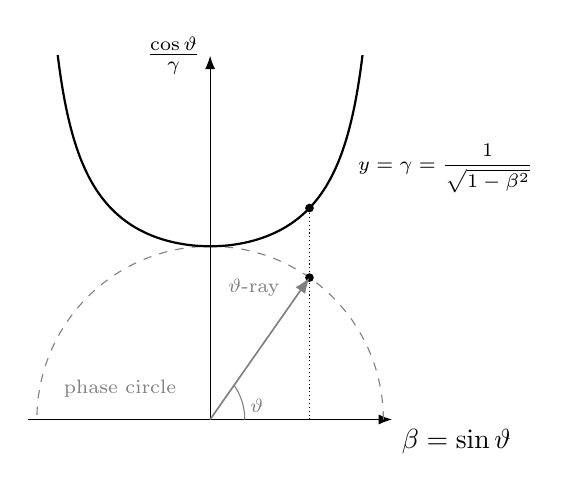
\begin{tikzpicture}[scale=2.2, >=Latex]
  % общие параметры
  \def\ymax{2.1}
  \def\th{35} % пример угла
  \pgfmathsetmacro{\bet}{sin(\th)}   % β = sin θ
  \pgfmathsetmacro{\co}{cos(\th)}    % cos θ
  \pgfmathsetmacro{\ga}{1/\co}       % γ = sec θ

  % оси (вне clip, чтобы надписи не резались)
  \draw[->] (-1.05,0) -- (1.05,0) node[below right] {$\beta=\sin\vartheta$};
  \draw[->] (0,0) -- (0,\ymax) node[left] {$\frac{\cos\vartheta}{ \gamma}$};

  \begin{scope}
    \clip (-1.05,0) rectangle (1.95,\ymax);

    \draw[gray,dashed] (0,0) circle (1);

    \draw[line width=0.8pt] plot[domain=-0.90:0.90, samples=240] (\x, {1/sqrt(1-\x*\x)});

    \draw[densely dotted] (\bet,0) -- (\bet,\ga);
    \fill (\bet,\co) circle (0.025);
    \fill (\bet,\ga) circle (0.025);
  \end{scope}

  \draw[gray,->,line width=0.6pt] (0,0) -- (\bet,\co) node[pos=0.8, above left] {\scriptsize $\vartheta$-ray};
  \draw[gray] (0.20,0) arc[start angle=0, end angle=\th, radius=\th/100];
  \node[gray] at (0.27,0.08) {\scriptsize $\vartheta$};

  \node[gray] at (-0.52,0.18) {\scriptsize phase circle};
  \node at (1.36,1.45) {\scriptsize $y=\gamma=\dfrac{1}{\sqrt{1-\beta^{2}}}$};
\end{tikzpicture}
\caption{Phase circle vs. Lorentz hyperbola at common $\beta=\sin\vartheta$. Vertical mapping at fixed $\beta$ illustrates the Gudermann bridge: $\gamma=\sec\vartheta=\cosh\eta$.}
\label{fig:circle-hyperbola-gd}
\end{figure}
\FloatBarrier

%5 ===================================================================

\section{Phase space}

We represent a flow state on a quaternionic \emph{complex slice}
$\mathbb C_{\mathbf u}:=\mathrm{Span}\{1,\mathbf u\}\subset\mathbb H$,
where $\mathbf u\in S^2$ is the unit spatial direction selected by the observer’s split.
The unit rotor on this slice is
\[
\widehat q(\vartheta,\mathbf u):=\cos\vartheta+\mathbf u\,\sin\vartheta\in S^3\simeq SU(2),
\]
and, under the calibration $\|\boldsymbol\chi\|\equiv \clight$ (cf.\ §\ref{sec:calibration-c}),
we parameterize the flow vector as
\begin{equation}
\boldsymbol\chi(\vartheta,\mathbf u)=\clight\,\widehat q(\vartheta,\mathbf u)
=\clight\bigl(\cos\vartheta+\mathbf u\,\sin\vartheta\bigr).
\label{eq:phase-rotor-chi}
\end{equation}

\paragraph{Phase-rate projections (observer $A$).}\label{sec:phase-rates}
Given an observer $A$ with split $(\mathbf e_t^A,S^A)$ and
observer–object angle $\vartheta_{|\!A}$ (see \S\ref{sec:minkowski-derivation}),
the phase-rate components with respect to $A$ are
\begin{equation}
\tilde X^0_{|\!A}:=\frac{dx^0_{|\!A}}{d\chi}
=\clight\,\cos\vartheta_{|\!A},\qquad
\tilde{\mathbf X}_{|\!A}:=\frac{d\mathbf x_{|\!A}}{d\chi}
=\clight\,\sin\vartheta_{|\!A}\,\mathbf u_{|\!A},
\label{eq:phase-rates}
\end{equation}
where $\mathbf u_{|\!A}:=P_{S^A}\widehat{\mathbf F}/\|P_{S^A}\widehat{\mathbf F}\|\in S^A$ is the unit spatial
direction as seen by $A$ and $\widehat{\mathbf F}:=\boldsymbol\chi/\|\boldsymbol\chi\|$.

These rates satisfy the identity
\begin{equation}
\Bigl(\frac{ds}{d\chi}\Bigr)^2
=\bigl(\tilde X^0_{|\!A}\bigr)^2-\bigl\|\tilde{\mathbf X}_{|\!A}\bigr\|^2
=\clight^2\bigl(1-\sin^2\vartheta_{|\!A}\bigr)
=\clight^2\cos^2\vartheta_{|\!A}.
\label{eq:phase-budget-identity}
\end{equation}
which, in the SR simplification ($\zeta=\phi=0$ and $dt_A:=d\chi$), is just the operational split
of the fixed budget $\clight$ into temporal/spatial projections.

\paragraph{Phase-to-observable map (integral form).}
For any chart $x^i$ adapted to $A$ we have the integral transform
\begin{equation}
x^i(\chi)=x^i(\chi_0)+\int_{\chi_0}^{\chi}\tilde X^i_{|\!A}(u)\,du,
\qquad i=0,1,2,3,
\label{eq:phase-integral-map}
\end{equation}
with $\tilde X^0_{|\!A}$ and $\tilde{\mathbf X}_{|\!A}$ from \eqref{eq:phase-rates}. In the SR sector
this becomes
\(
t_A(\chi)=t_A(\chi_0)+\int_{\chi_0}^{\chi} du
\)
and
\(
\mathbf x_{|\!A}(\chi)=\mathbf x_{|\!A}(\chi_0)
+\int_{\chi_0}^{\chi}\clight\,\sin\vartheta_{|\!A}(u)\,\mathbf u_{|\!A}(u)\,du.
\)

\paragraph{Intrinsic vs.\ directional factors.}
The intrinsic second-moment angle $\zeta$ (\S\ref{sec:intrinsic-angle}) enters the body’s own
rate via $d\tau_B/d\chi=\cos\zeta$, while \eqref{eq:phase-rates} is purely directional and built
from the observer’s split. Outside the SR sector the intrinsic interval is
$ds_B^2=\clight^2\cos^2\zeta\,d\chi^2-d\boldsymbol\ell^{\!\top}\mathbf C_B\,d\boldsymbol\ell$,
and \eqref{eq:phase-integral-map} remains valid as a kinematic reconstruction of observables from
phase rates.

%6 ===================================================================
\section{Objects: operational catalogue and inference}
\label{sec:objects-catalogue}

\paragraph{Scope.} This section is a look-up summary. The physics and proofs live in
\S\ref{sec:body}, \S\ref{sec:intrinsic-angle}, \S\ref{sec:calibration-c}, and \S\ref{sec:phase-deriv}.

\subsection*{Canonical cases}
\begin{enumerate}
\item \textbf{Photon (vacuum).} \(\,T_B=0,\ d\tau_B=0,\ \|d\boldsymbol\ell\|/d\chi=\clight\) (Def.~\eqref{eq:calib-null}).
\item \textbf{Massive isotropic body.} \(\,\mathbf C_B=\frac{\sin^2\zeta}{3}\mathbf I,\quad
d\tau_B=\cos\zeta\,d\chi,\quad ds_B^2=\clight^2\cos^2\zeta\,d\chi^2-\frac{\sin^2\zeta}{3}\|d\boldsymbol\ell\|^2.\)
\item \textbf{Anisotropic body.} \(\,\mathbf C_B=\sum_{i=1}^3 \lambda_i\,\hat{\mathbf e}_i\otimes\hat{\mathbf e}_i,\ 
\lambda_i\ge0,\ \sum_i\lambda_i=\sin^2\zeta.\) Pullbacks along \(\hat{\mathbf e}_i\) probe \(\lambda_i\).
\item \textbf{Effective medium (\(\zeta\) only).} \(\,d\tau/dt=\cos\zeta,\ n(\zeta)=\sec\zeta\) (cf.\ \S\ref{ch:optics}).
\end{enumerate}

\subsection*{Parameter inference}
\begin{itemize}
\item \emph{Rate split at rest.} With \(\vartheta=0,\ \phi=0\): \(\cos\zeta=\bigl(d\tau_B/dt\bigr)_{\text{meas}}\).
\item \emph{Directional pullbacks.} Measure \(ds_B^2\) for small \(d\boldsymbol\ell\) along several lab directions;
fit the quadratic form \(q_B=d\boldsymbol\ell^\top\mathbf C_B\,d\boldsymbol\ell\Rightarrow\) eigenpairs \((\lambda_i,\hat{\mathbf e}_i)\).
\item \emph{Factorization with gravity/kinematics.} Use \(d\tau/dt=\cos\zeta\cos\phi\cos\vartheta\) to separate
\(\phi\) (clock angle) from \(\zeta\) via e.g.\ static vs moving protocols (see \S\ref{ch:optics}).
\end{itemize}

\subsection*{Ensemble composition}
For streamlets \(a\) with weights \(w_a\): \(T_B=\sum_a w_a\cos^2\Theta_a,\ 
\mathbf C_B=\sum_a w_a\sin^2\Theta_a\,\mathbf u_a\otimes\mathbf u_a\) (Eq.\ \eqref{eq:TB-CB}).

\subsection*{Non-collinear boosts}
Composition induces a spatial Wigner rotation on orientations without altering the scalar rate factorization;
see \S\ref{subsec:wigner}, \S\ref{subsec:thomas}.


%7 ===================================================================

\section{\texorpdfstring{Phase-derivative view}{Phase-derivative view}}
\label{sec:phase-deriv}

\noindent\textit{Scope.} This section repackages core identities in the language of
\emph{phase derivatives}, using only notions already introduced
(\S\ref{sec:calibration-c}–\ref{sec:minkowski-derivation}). No new kinematics is postulated.

\paragraph{Notation recap (from \S\ref{sec:phase-rates}).}
Phase–rate components for an observer $A$ are
\begin{equation}
\tilde X^0_{|\!A}=\frac{dx^0_{|\!A}}{d\chi}=\clight\,\cos\vartheta_{|\!A},\qquad
\tilde{\mathbf X}_{|\!A}=\frac{d\mathbf x_{|\!A}}{d\chi}
=\clight\,\sin\vartheta_{|\!A}\,\mathbf u_{|\!A},
\tag{\ref{eq:phase-rates}}
\end{equation}
and obey the identity
\begin{equation}
\Bigl(\frac{ds}{d\chi}\Bigr)^2
=\bigl(\tilde X^0_{|\!A}\bigr)^2-\bigl\|\tilde{\mathbf X}_{|\!A}\bigr\|^2
=\clight^2\bigl(1-\sin^2\vartheta_{|\!A}\bigr)
=\clight^2\cos^2\vartheta_{|\!A}.
\tag{\ref{eq:phase-budget-identity}}
\end{equation}
A change of parameter $\chi\mapsto\tau$ acts by the Jacobian $\mathcal J:=\dfrac{d\chi}{d\tau}$:
\begin{equation}
\dot X^i=\frac{d x^i}{d\tau}=\mathcal J\,\tilde X^i,\qquad
\dot{X}\equiv d/d\tau,\quad \tilde{X}\equiv d/d\chi.
\label{eq:param-change}
\end{equation}

\subsection{Minkowski–phase equality of invariants}
\label{subsec:phase-minkowski-equality}

\textbf{Theorem.} For any worldline segment and any observer $A$,
\begin{equation}
\boxed{\ \tilde H \;=\; \dot S\ },\qquad
\tilde H^2:=\bigl(\tilde X^0_{|\!A}\bigr)^2+\bigl\|\tilde{\mathbf X}_{|\!A}\bigr\|^2,\quad
\dot S^2:=\bigl(\dot X^0_{|\!A}\bigr)^2-\bigl\|\dot{\mathbf X}_{|\!A}\bigr\|^2 .
\label{eq:phase-minkowski-equality}
\end{equation}

\emph{Proof.} By \eqref{eq:param-change},
$\dot X^i=\mathcal J\,\tilde X^i$, hence
\[
\dot S^2=(\mathcal J\tilde X^0)^2-\|\mathcal J\tilde{\mathbf X}\|^2
=\mathcal J^2\!\left(\tilde X^0{}^2-\|\tilde{\mathbf X}\|^2\right)
=\mathcal J^2\Bigl(\frac{ds}{d\chi}\Bigr)^2
=\Bigl(\frac{ds}{d\tau}\Bigr)^2.
\]
At the same time,
$\tilde H^2=\tilde X^0{}^2+\|\tilde{\mathbf X}\|^2
=\clight^2$ in the SR gauge (\S\ref{subsec-1-5-sr-simplification}),
and $ds/d\tau=\clight$ by the operational split
$\cos\vartheta=d\tau/dt$, $\sin\vartheta=\|\mathbf v\|/\clight$ (\S\ref{sec:operational-phase}).
Therefore $\tilde H=\dot S=\clight$. $\square$

\paragraph{Reading.} In words: the Euclidean norm of the phase–rate vector equals the Minkowski
norm of the observable rate vector. The equality \eqref{eq:phase-minkowski-equality} is the
derivative form of “the same budget seen in two parametrizations”.

\subsection{Photon time: null interval and phase parameter}
\label{subsec:photon-phase-time}

For a lightlike flow in vacuum, the body’s intrinsic quadratic form gives
$ds_B^2=0$ (\S\ref{sec:calibration-c}), hence the body-level proper increment vanishes:
\begin{equation}
\boxed{\ d\tau_B=0\quad\text{(null flow, vacuum)}\ }.
\label{eq:photon-null}
\end{equation}
Nevertheless the phase parameter $\chi$ advances and serves as an \emph{affine} parameter along
the ray. With the calibration \eqref{eq:calib-null} we have
\begin{equation}
\frac{\|d\boldsymbol\ell\|}{d\chi}=\mathtt c,\qquad
\Rightarrow\quad \chi=\text{(cycle counter)}.
\label{eq:photon-affine}
\end{equation}

Under the convention $\Phi=\omega\,\chi$, one cycle corresponds to $\Delta\chi=2\pi/\omega$, so $\chi$ counts
wavefronts affinely while the intrinsic metric remains null ($d\tau_B=0$).


At unit frequency, $\nu:=d\chi/d\tau=1$, the phase equals the proper-time parameter used as an
affine label of wavefronts; no contradiction with \eqref{eq:photon-null} arises because
$\tau$ here is a \emph{chosen} parameter for counting cycles, while the intrinsic
metric length remains null.

% --- PATCH: insert after § Mapping to SR (before or after the correspondences table) ---

\subsection{Relativistic Doppler as a phase–kinematic theorem}\label{sec:doppler-core}

We derive the Doppler law purely from the phase split, without hyperbolic parametrization or dynamics.

\paragraph{Setup.}
Define frequency as the phase growth rate in proper time,
\(
\nu:=d\chi/d\tau
\),
and consider two successive wavefronts separated by the same phase increment
\(
\Delta\chi
\)
for the source and the observer. Then
\begin{equation}
\frac{\nu_{\mathrm{obs}}}{\nu_{\mathrm{src}}}
=\frac{d\chi/d\tau_{\mathrm{obs}}}{d\chi/d\tau_{\mathrm{src}}}
=\frac{d\tau_{\mathrm{src}}}{d\tau_{\mathrm{obs}}}.
\label{eq:doppler-core-master}
\end{equation}

In the SR sector (\(\zeta=\phi=0\)) the observer at rest has \(d\tau_{\mathrm{obs}}=dt_{\mathrm{obs}}\),
and for the (possibly moving) source \(dt_{\mathrm{src}}=\gamma\,d\tau_{\mathrm{src}}\) with
\(\gamma=\sec\vartheta\), \(\beta=\sin\vartheta\).

\paragraph{Longitudinal case.}
During the emission interval \(dt_{\mathrm{src}}=\gamma\,d\tau_{\mathrm{src}}\) (measured in the
observer’s lab chart) the source shifts by \(\pm \beta c\,dt_{\mathrm{src}}\) along the line of sight
(“\(+\)” receding, “\(-\)” approaching). The reception interval is the emission interval plus the
change in light flight time:
\[
dt_{\mathrm{obs}}
= dt_{\mathrm{src}} \,\bigl(1\pm \beta\bigr)
= \gamma\,d\tau_{\mathrm{src}} \,\bigl(1\pm \beta\bigr).
\]
With \eqref{eq:doppler-core-master} and \(d\tau_{\mathrm{obs}}=dt_{\mathrm{obs}}\) this gives the Doppler factor
\begin{equation}
\boxed{\ \frac{\nu_{\mathrm{obs}}}{\nu_{\mathrm{src}}}
=\frac{1}{\gamma(1\pm\beta)}\ }
=\sqrt{\frac{1\mp\beta}{1\pm\beta}}
=\sec\vartheta\,(1\mp\sin\vartheta)
=e^{\mp\eta},
\label{eq:doppler-core-long}
\end{equation}
where the equivalent forms use \(\beta=\sin\vartheta\), \(\gamma=\sec\vartheta\), and the Gudermann bridge \eqref{eq:gudermann}.

\paragraph{Transverse case.}
For \(\varphi=90^\circ\) (emission orthogonal to the relative velocity in the observer’s frame),
the geometric flight-time correction vanishes, hence
\begin{equation}
\boxed{\ \frac{\nu_{\mathrm{obs}}}{\nu_{\mathrm{src}}}=\frac{1}{\gamma}=\cos\vartheta\ }.
\label{eq:doppler-core-trans}
\end{equation}

\paragraph{General line-of-sight angle.}
Let \(\varphi\) be the angle between the source velocity and the line of sight in the observer’s frame.
Only the LOS component \(\beta\cos\varphi\) changes the flight time; repeating the above,
\begin{equation}
\boxed{\ \frac{\nu_{\mathrm{obs}}}{\nu_{\mathrm{src}}}
=\frac{1}{\gamma\,(1-\beta\cos\varphi)}
\ =\ \gamma\,(1-\beta\cos\varphi)^{-1}\ }.
\label{eq:doppler-core-los}
\end{equation}
Equivalently, in phase variables,
\(\nu_{\mathrm{obs}}/\nu_{\mathrm{src}}=\sec\vartheta\,\bigl(1-\sin\vartheta\cos\varphi\bigr)^{-1}\).

\paragraph{Corollary (with intrinsic/gravitational tilts).}
Outside the pure SR sector, the total redshift factorizes:
\[
1+z_{\rm tot}
=\frac{\nu_{\mathrm{src}}}{\nu_{\mathrm{obs}}}
=\underbrace{\gamma(1-\beta\cos\varphi)}_{\text{kinematic}}
\,\times\,
\underbrace{\frac{\cos\zeta_{\rm obs}\cos\phi_{\rm obs}}{\cos\zeta_{\rm src}\cos\phi_{\rm src}}}_{\text{intrinsic \& gravitational}},
\]
which reproduces \eqref{eq:z-factorization} upon identifying the kinematic part with
\eqref{eq:doppler-core-los}.

\paragraph{Infinitesimal form (longitudinal).}
Taking the differential of $\ln(\nu_{\mathrm{obs}}/\nu_{\mathrm{src}})$,
\begin{equation}
\boxed{\ d\ln\frac{\nu_{\mathrm{obs}}}{\nu_{\mathrm{src}}}
= \mp\,d\eta
= \mp\,\sec\vartheta\,d\vartheta
= \mp\,\gamma^{2}\,d\beta\ },
\label{eq:doppler-inf-long}
\end{equation}
with the upper sign for receding (“$+$” in \eqref{eq:doppler-finite-deriv}) and lower for approaching.
Equation \eqref{eq:doppler-inf-long} is the \emph{phase–derivative} Doppler law.

\paragraph{Transverse case.}
For $\varphi=90^\circ$ in the observer’s frame the flight-time correction vanishes,
so $\nu_{\mathrm{obs}}/\nu_{\mathrm{src}}=1/\gamma$ and
\begin{equation}
d\ln\frac{\nu_{\mathrm{obs}}}{\nu_{\mathrm{src}}}=-\,d\ln\gamma=-\beta\gamma^2\,d\beta.
\label{eq:doppler-inf-trans}
\end{equation}

\paragraph{General LOS angle (fixed geometry).}
If $\varphi$ is the angle between the velocity and the line of sight in the observer’s frame and
$d\varphi=0$, then from
$\nu_{\mathrm{obs}}/\nu_{\mathrm{src}}=1/\bigl[\gamma(1-\beta\cos\varphi)\bigr]$ one gets
\begin{equation}
d\ln\frac{\nu_{\mathrm{obs}}}{\nu_{\mathrm{src}}}
=-\Bigl[\beta\gamma^2-\frac{\cos\varphi}{1-\beta\cos\varphi}\Bigr]\,d\beta
\ =\ -\,d\eta\ \ \text{when }\ \varphi=0,\pi .
\label{eq:doppler-inf-los}
\end{equation}

\medskip
Together, \eqref{eq:phase-minkowski-equality}, \eqref{eq:photon-null}–\eqref{eq:photon-affine}, and
\eqref{eq:doppler-inf-long}–\eqref{eq:doppler-inf-los} show how \emph{phase derivatives} encode:
(i) equality of observable and phase invariants;
(ii) the null nature of photon proper time with $\chi$ as an affine counter;
(iii) the Doppler law, both finite and in instantaneous differential form.

%8 ===================================================================

\section{Unified temporal effects in phase space}
\label{ch:optics}

We factor all time-related effects through a single phase tilt structure.
Let the intrinsic (\(\zeta\)), gravitational (\(\phi\)), and kinematic (\(\vartheta\)) angles be independent contributors to the phase tilt at a point.
Define the local \emph{time-rate factor}
\begin{equation}
\label{eq:time-rate-factor}
\frac{d\tau}{dt}
\;=\;
\cos\zeta\;\cos\phi\;\cos\vartheta,
\qquad
n_{\rm tot}\;:=\;\sec\zeta\;\sec\phi\;\sec\vartheta,
\end{equation}
where \(n_{\rm tot}\) plays the role of an effective (phase) refractive index for light propagation.
Accordingly, the coordinate light-travel time along a spatial curve \(\Gamma\) is
\begin{equation}
\label{eq:optical-length}
t_\Gamma \;=\; \frac{1}{\clight}\int_\Gamma n_{\rm tot}\,ds.
\end{equation}

\paragraph{Lemma (Unified time-rate).}
In the unimetry phase representation, the proper-to-lab time rate and the optical length factorize as in \eqref{eq:time-rate-factor}–\eqref{eq:optical-length}.
Setting any subset of angles to zero recovers the corresponding standard effects:
\begin{itemize}\itemsep4pt
  \item \textbf{Special relativity (vacuum SR):} \(\zeta=0,\ \phi=0\Rightarrow d\tau/dt=\cos\vartheta=1/\gamma\) (kinematic time dilation).
  \item \textbf{Gravitational clocks (static weak field):} \(\zeta=0,\ \vartheta=0\Rightarrow d\tau/dt=\cos\phi\) (gravitational redshift/clock rate); calibration of \(\phi\) reproduces the usual \(\sqrt{g_{00}}\).
  \item \textbf{Shapiro delay (gravitational contribution to TOF):} with \(\zeta=0,\ \vartheta=0\), \eqref{eq:optical-length} yields \(t_\Gamma=(1/\clight)\int \sec\phi\,ds\); the excess over \(\int ds/\clight\) is the Shapiro time delay.
  \item \textbf{Intrinsic/evolutionary tilt:} \(\phi=0,\ \vartheta=0\Rightarrow d\tau/dt=\cos\zeta,\ n_{\rm tot}=\sec\zeta\) (useful as a time gauge in cosmological/effective-medium contexts).
\end{itemize}

\paragraph{Remarks.}
(i) The factorization in \eqref{eq:time-rate-factor} is the phase-space counterpart of composing independent tilts; it preserves the conserved Minkowski norm once time is reparameterized by \(\tau\).
(ii) For vacuum SR we simply set \(\zeta=0\) and work with \(\vartheta\); for pure gravitational timing we set \(\vartheta=0\) and use \(\phi\).
(iii) Non-collinear boost composition acts on \(\vartheta\) via quaternionic rotors and induces a Wigner/Thomas residual \emph{spatial} rotation without altering \eqref{eq:time-rate-factor}.

%9 ===================================================================

\section{\texorpdfstring{Gravity as a phase rotation: local tetrads and clock angle}{Gravity as a phase rotation}}

On a curved background $(\mathcal M,g)$ we work with orthonormal tetrads $e_a{}^\mu$ such that $g_{\mu\nu}e_a{}^\mu e_b{}^\nu=\eta_{ab}$ and take the observer's time leg to be $e_0{}^\mu$. 
We apply the gravitational (clock) angle $\phi$ as
\begin{equation}
\cos\phi\ :=\ e^0{}_\mu\,u^\mu\ =\ \frac{d\tau_{\rm stat}}{dt}\ =\ \sqrt{-g_{00}}\qquad\text{(stationary case)}.
\label{eq:clock-angle}
\end{equation}

Kinematics remains encoded by the phase angle $\vartheta$ in the slice $\mathbb C_{\mathbf u}$, with
$\cos\vartheta=d\tau/d\tau_{\rm stat}$. 
Therefore the proper time factorizes as
\begin{equation}
d\tau\ =\ dt\,\cos\phi\,\cos\vartheta,\qquad 
d\mathbf x\ =\ c\,dt\,\sin\vartheta\,\mathbf u,
\label{eq:tau-factorization}
\end{equation}
and the total redshift factorizes into kinematic and gravitational parts:
\begin{equation}
1+z_{\rm tot}\ =\ \frac{\cos\vartheta_{\rm em}}{\cos\vartheta_{\rm obs}}\ \times\ 
\frac{\cos\phi(x_{\rm em})}{\cos\phi(x_{\rm obs})}.
\label{eq:z-factorization}
\end{equation}

For static emitter/observer ($\vartheta_{\rm em}=\vartheta_{\rm obs}=0$) one recovers the standard gravitational redshift 
$1+z_g=\sqrt{\frac{-g_{00}(x_{\rm obs})}{-g_{00}(x_{\rm em})}}$.
In the weak-field limit $g_{00}\simeq-(1+2\Phi/c^2)$ this gives $z_g\simeq(\Phi_{\rm obs}-\Phi_{\rm em})/c^2$.

\paragraph{Beyond static fields.}
In a $3\!+\!1$ split $ds^2=-N^2 c^2 dt^2 + h_{ij}(dx^i+N^i dt)(dx^j+N^j dt)$ one may identify $\cos\phi:=N$ in the observer's tetrad, which keeps \eqref{eq:tau-factorization}–\eqref{eq:z-factorization} coordinate-agnostic.
Uniform acceleration (Rindler) accumulates phase according to $d\vartheta=\kappa\,dt$ inside the local slice, consistently reproducing accelerated-frame kinematics when combined with the clock angle $\phi$.

%9 ===================================================================
\section*{Outlook}

The unimetry framework developed here provides a versatile foundation for future theoretical developments in both relativity and quantum physics. The following directions emerge as particularly promising:
\begin{itemize}
    \item
    \textbf{Extension to General Relativity.} The modular phase decomposition is well suited for the introduction of curved metrics, potentially allowing gravitational redshift, time delay (Shapiro effect), and even curvature-driven precessions to be recast in the language of phase tilts and generalized rotors. Realizing Einstein's dynamics for gravitational fields in this formalism is a natural next step, especially via the local tetrad and clock angle structures already sketched.

    \item
    \textbf{Quantum Connections.} Given the central role of phase, rotors, and symmetry groups (notably the demonstration of Hopf fibration structure), the unimetry formalism can serve as a stepping stone toward a deeper unification between relativistic and quantum frameworks, possibly via geometric quantization or generalized qubit/Bloch-sphere analogues.

    \item
    \textbf{Physical and Experimental Applications.} The structure is already suited for reinterpretation and numerical simulation of phenomena involving non-collinear accelerations, such as in advanced particle beam physics or optical systems with phase media. This computational potential deserves further methodological and comparative exploration.

    \item
    \textbf{Generalizations and Group Theory.} The embedding of Lorentzian kinematics within a more general Euclidean group-theoretic framework (potentially encompassing de Sitter or conformal transformations) may suggest further extensions, including nontrivial topologies, higher dimensions, or self-dual (instanton-like) solutions.
\end{itemize}

In summary, by replacing the traditional spacetime paradigm with a geometric flow in phase space, unimetry opens avenues for new mathematical structures and connections among relativity, geometry, and quantum theory. Its broader success will depend on future progress in developing the gravitational and quantum sectors and on the demonstration of concrete computational and experimental advantages.





\bibliographystyle{plain}
\begin{thebibliography}{9}
\bibitem{Gudermann1830}  NIST Digital Library of Mathematical Functions, §4.23 ``Gudermannian Function'', \url{https://dlmf.nist.gov/4.23}.

\bibitem{Hopf1931}
H.~Hopf, ``Über die Abbildungen der dreidimensionalen Sphäre auf die Kugelfläche,'' \emph{Mathematische Annalen} \textbf{104} (1931) 637--665. \href{https://doi.org/10.1007/BF01457962}{doi:10.1007/BF01457962}.

\bibitem{Thomas1926}
L.~H.~Thomas, ``The Motion of the Spinning Electron,'' \emph{Nature} \textbf{117} (1926) 514. \href{https://doi.org/10.1038/117514a0}{doi:10.1038/117514a0}.

\bibitem{Wigner1939}
E.~P.~Wigner, ``On Unitary Representations of the Inhomogeneous Lorentz Group,'' \emph{Annals of Mathematics} \textbf{40} (1939) 149--204. \href{https://doi.org/10.2307/1968551}{doi:10.2307/1968551}.
\bibitem{Berry1984}
M.~V.~Berry, ``Quantal phase factors accompanying adiabatic changes,'' \emph{Proceedings of the Royal Society A} \textbf{392} (1984) 45--57. \href{https://doi.org/10.1098/rspa.1984.0023}{doi:10.1098/rspa.1984.0023}.

\bibitem{Shapiro1964}
I.~I.~Shapiro, ``Fourth Test of General Relativity,'' \emph{Phys. Rev. Lett.} \textbf{13} (1964) 789--791. \href{https://doi.org/10.1103/PhysRevLett.13.789}{doi:10.1103/PhysRevLett.13.789}.

\bibitem{RindlerBook}
W.~Rindler, \emph{Relativity: Special, General, and Cosmological}, 2nd ed., Oxford University Press, 2006.

\bibitem{MTW}
C.~W.~Misner, K.~S.~Thorne, J.~A.~Wheeler, \emph{Gravitation}, W.~H.~Freeman, 1973.

\bibitem{Jackson}
J.~D.~Jackson, \emph{Classical Electrodynamics}, 3rd ed., Wiley, 1999.

\bibitem{Einstein1905}
A.~Einstein.
\newblock Zur Elektrodynamik bewegter K\"{o}rper.
\newblock {\em Annalen der Physik}, 17:891--921, 1905.
(English translation: On the electrodynamics of moving bodies.)

\bibitem{Rindler}
W.~Rindler.
\newblock {\em Relativity: Special, General, and Cosmological}.
\newblock Oxford University Press, 2nd ed., 2006.

\bibitem{TaylorWheeler}
E.~F. Taylor and J.~A. Wheeler.
\newblock {\em Spacetime Physics}.
\newblock W. H. Freeman, 2nd ed., 1992.

\bibitem{Hamilton1844}
W.~R.~Hamilton,
\newblock \emph{On quaternions; or on a new system of imaginaries in algebra}, Philosophical Magazine \textbf{25}, 10--13 (1844).

\bibitem{HestenesSobczyk1984}
D.~Hestenes and G.~Sobczyk,
\newblock \emph{Clifford Algebra to Geometric Calculus}, Reidel, 1984.

\bibitem{DoranLasenby2003}
C.~Doran and A.~Lasenby,
\newblock \emph{Geometric Algebra for Physicists}, Cambridge University Press, 2003.

\end{thebibliography}




\appendix
\section{Equivalence to the classical Wigner rotation}
\label{app:1}

We sketch an intrinsic quaternionic proof that the unimetry expression for the Wigner rotation
coincides with the standard special-relativistic formula.

\paragraph{Step 1: product of two D-rotors.}
For $d_i=\cos\frac{\psi_i}{2}+\uhat_i\sin\frac{\psi_i}{2}$,
\begin{equation}
\label{eq:auto:45}
d_2 d_1
=(c_2c_1-s_2s_1\cos\theta)
+\Big(c_2s_1\uhat_1+s_2c_1\uhat_2+s_2s_1\,\uhat_2\times\uhat_1\Big),
\end{equation}
with $c_i=\cos(\psi_i/2)$, $s_i=\sin(\psi_i/2)$ and $\cos\theta=\uhat_2\!\cdot\!\uhat_1$.

\paragraph{Step 2: symmetric D--R factorization.}
Define $d_{12}$ by $d_{12}\,\mathbf e_t\, d_{12}=L_{12}\,\mathbf e_t\, L_{21}$ and set
$r_W=\bar d_{12}\,L_{12}=L_{21}\,\bar d_{12}$. Then $r_W$ fixes $\mathbf e_t$ and is a pure spatial
rotor, so $r_W=\cos\frac{\phi}{2}+\hat{\mathbf n}\sin\frac{\phi}{2}$ with
$\hat{\mathbf n}\parallel \uhat_2\times\uhat_1$. Matching scalar and bivector parts gives
\begin{equation}
\tan\frac{\phi}{2}=
\frac{s_1 s_2\,\sin\theta}{\,c_1 c_2+s_1 s_2\,\cos\theta\,}.
\label{eq:uni-phi}
\end{equation}

\paragraph{Step 3: map to rapidities.}
With the substitutions $\sin(\psi/2)\mapsto\sinh(\eta/2)$, $\cos(\psi/2)\mapsto\cosh(\eta/2)$,
$\tan(\psi/2)\mapsto\tanh(\eta/2)$ (where $\tanh\eta=\beta$, $\cosh\eta=\gamma$), \eqref{eq:uni-phi}
becomes the textbook Wigner angle:
\begin{equation}
\label{eq:auto:47}
\tan\frac{\phi}{2}
=\frac{\sinh\frac{\eta_1}{2}\,\sinh\frac{\eta_2}{2}\,\sin\theta}
{\cosh\frac{\eta_1}{2}\,\cosh\frac{\eta_2}{2}+\sinh\frac{\eta_1}{2}\,\sinh\frac{\eta_2}{2}\,\cos\theta},
\end{equation}
with axis along $\uhat_2\times\uhat_1$. This circular--hyperbolic correspondence is classical; cf.\ Gudermann~\cite{Gudermann1830}.

\section{A worked example — Wigner angle in hyperbolic vs phase parametrizations with a stability note}\label{app:wigner}
\label{app:2}

\paragraph{Closed-form formulae.}
Let $\boldsymbol\beta_i$ ($i=1,2$) be two non-collinear boost velocities with magnitudes $\beta_i=\|\boldsymbol\beta_i\|<1$ and let $\chi$ be the angle between their \emph{directions}.
The Thomas–Wigner rotation $R_W$ generated by the composition of boosts has axis
$\hat{\mathbf n}\parallel \hat{\boldsymbol\beta}_2\times \hat{\boldsymbol\beta}_1$
and angle $\psi_W$ given by either of the following equivalent half–angle forms:
\begin{align}
\tan\frac{\psi_W}{2}
&=\frac{\sin\chi\;\tanh\!\frac{\eta_1}{2}\;\tanh\!\frac{\eta_2}{2}}
       {1+\cos\chi\;\tanh\!\frac{\eta_1}{2}\;\tanh\!\frac{\eta_2}{2}} ,
\qquad \beta_i=\tanh\eta_i ,
\label{eq:wigner-hyp}\\[4pt]
\tan\frac{\psi_W}{2}
&=\frac{\sin\chi\;\tan\!\frac{\vartheta_1}{2}\;\tan\!\frac{\vartheta_2}{2}}
       {1+\cos\chi\;\tan\!\frac{\vartheta_1}{2}\;\tan\!\frac{\vartheta_2}{2}} ,
\qquad \beta_i=\sin\vartheta_i .
\label{eq:wigner-phase}
\end{align}
Numerically stable and parametrization–agnostic is the identity
\begin{equation}
\tanh\!\frac{\eta_i}{2}=\tan\!\frac{\vartheta_i}{2}
=\frac{\gamma_i\beta_i}{1+\gamma_i}
=\frac{\beta_i}{\,1+\sqrt{1-\beta_i^2}\,}
=:t_i ,
\qquad \gamma_i=(1-\beta_i^2)^{-1/2}.
\label{eq:half-angle-t}
\end{equation}
With $t_i$ from \eqref{eq:half-angle-t}, both \eqref{eq:wigner-hyp}–\eqref{eq:wigner-phase} reduce to
\begin{equation}
\psi_W
=2\,\operatorname{atan2}\!\Big(\sin\chi\,t_1t_2,\;1+\cos\chi\,t_1t_2\Big),
\label{eq:wigner-atan2}
\end{equation}
which avoids overflow/underflow and ensures the correct quadrant.

\paragraph{Example A (orthogonal boosts, moderate $\gamma$).}
Take $\boldsymbol\beta_1=(0.8,0,0)$ and $\boldsymbol\beta_2=(0,0.6,0)$, so $\chi=\pi/2$.
From \eqref{eq:half-angle-t} one finds $t_1=\tfrac{1}{2}$ and $t_2=\tfrac{1}{3}$ exactly,
hence $\tan(\psi_W/2)=t_1t_2=\tfrac{1}{6}$ and
\[
\boxed{\;\psi_W
=2\arctan\!\frac{1}{6}
=0.3302973548292537~\text{rad}
=18.924644416051237^\circ\;}
\]
Both parametrizations \eqref{eq:wigner-hyp} and \eqref{eq:wigner-phase} coincide to machine precision.
A direct $4{\times}4$ Lorentz–matrix composition followed by polar decomposition of the spatial block
recovers $\psi_W=0.3302973548292533$ rad (agreement to $<5{\times}10^{-16}$ rad).

\paragraph{Example B (ultra–relativistic, small inter–direction angle).}
Let $\boldsymbol\beta_1=(0.999999,0,0)$ and
$\boldsymbol\beta_2=0.9999(\cos 1^\circ,\sin 1^\circ,0)$ so that $\chi=1^\circ$.
Then \eqref{eq:half-angle-t} gives $t_1=0.9985867853779378$, $t_2=0.9859568136154433$ and
\[
\boxed{\;\psi_W
=2\,\operatorname{atan2}\!\big( \sin1^\circ\;t_1t_2,\;1+\cos1^\circ\;t_1t_2\big)
=0.0173175319077011~\text{rad}
=0.9922214898944112^\circ\;}
\]
The same value is obtained from either \eqref{eq:wigner-hyp} or \eqref{eq:wigner-phase}.
A double–precision Lorentz–matrix calculation with orthonormalization of the spatial block yields
$\psi_W=0.0173175044768120$ rad (agreement to $\sim 3{\times}10^{-8}$ rad; the residual is purely numerical).

\paragraph{Stability and accumulated error (practical note).}
\begin{itemize}
\item \textbf{Half–angle is key.} Computing via \eqref{eq:half-angle-t} and \eqref{eq:wigner-atan2} is markedly more stable than
naively evaluating $\eta_i=\operatorname{artanh}\beta_i$ followed by $\sinh(\eta_i/2),\cosh(\eta_i/2)$,
especially for $\gamma\gtrsim 10^2$ or tiny $\chi$ where subtractive cancellation appears in the denominator of \eqref{eq:wigner-hyp}.
\item \textbf{Single vs double precision.}
For Example~A, all routes (phase/hyperbolic/matrix) agree within $\sim 10^{-7}$ rad even in single precision.
For Example~B, the analytic half–angle formula \eqref{eq:wigner-atan2} remains well-behaved in single precision
($\psi_W=0.01731725$ rad; deviation $\sim 3{\times}10^{-7}$ rad),
while a direct $4{\times}4$ matrix composition in single precision becomes ill–conditioned (eigen–based orthonormalization fails to converge), a manifestation of catastrophic rounding at $\gamma\sim 10^3$.
\item \textbf{Error accumulation under repetitions.}
If the same pair of boosts is applied repeatedly, the rotation axis $\hat{\mathbf n}$ is fixed and the angle adds linearly mod $2\pi$.
In finite precision, composing dense Lorentz matrices $N$ times amplifies roundoff roughly linearly in $N$,
whereas evaluating \eqref{eq:wigner-atan2} per step and accumulating the angle avoids the growth of matrix–multiplication conditioning.
\end{itemize}

\paragraph{Recommendation (for reproducible numerics).}
Use \eqref{eq:half-angle-t} to form $t_i$ directly from $\beta_i$, then evaluate \eqref{eq:wigner-atan2} with \texttt{atan2}.
When a matrix route is unavoidable, extract the spatial rotation by removing the net boost and projecting the $3{\times}3$ block to $\mathrm{SO}(3)$ via a polar decomposition before reading off $\psi_W$.


\end{document}
